\documentclass[11pt,letterpaper]{article}
\usepackage[margin=1in]{geometry}
\usepackage{times}
\usepackage{booktabs}
\usepackage{graphicx}
\usepackage{microtype}
\usepackage{amsmath}
\usepackage{natbib}
\usepackage[hidelinks]{hyperref}

\title{Task Framing Outweighs Model Scale in Contract Clause Extraction:\\
Pre-Registered Experiments with Frontier LLMs and Small Fine-Tuned
Specialists on CUAD}
\author{Ashish Kumar Singh\\
\small\url{https://www.linkedin.com/in/ashish-kr-singh-ml/}}
\date{July 2026}

\begin{document}
\maketitle

\begin{abstract}
We benchmark four frontier language models (Claude Opus 4.8, Claude Opus 4.6,
GPT-5.2, GPT-4o) and a series of small fine-tuned specialists on CUAD contract
clause extraction, scored with the official AUPR metric through one identical
pipeline, with every raw prediction file published. Three findings emerge.
First, the frontier gap is category-shaped rather than uniform: a fine-tuned
14B specialist that trails the best frontier model by 17 points overall still
beats GPT-4o in 25 of 40 clause categories and beats all four frontier models
simultaneously in six. Second, task framing dominates model scale. Reframing
the specialist from answer generation to extractive span prediction, with the
base model, data, and budget held fixed, moves test AUPR from 0.291 to 0.389,
while growing the extractive backbone 28x (0.5B to 14B) moves dev AUPR only
from 0.284 to 0.303. Frontier scaling shows the same pattern: GPT-4o and
GPT-5.2, a full model generation apart, score within 0.002 of each other.
Third, we pre-registered a public prediction that the extractive 14B would
clear 0.50 test AUPR; it missed, and an analysis of the miss localizes the
remaining gap to the deliberately lean training recipe rather than
architecture or scale. Total specialist cost was about \$32 of GPU time
against roughly \$165 per frontier evaluation run. All code, predictions, and
the trained adapter are public.
\end{abstract}

\section{Introduction}

Contract review is one of the most commercially active applications of large
language models, and most deployed systems pay frontier API prices for it.
Clause extraction, the task of locating the span of a contract that evidences
a category such as governing law or a non-compete, is narrow, repetitive, and
convention-heavy. This is exactly the profile where a small fine-tuned
specialist should compete. Whether it actually does, and where, is an
empirical question that whole-benchmark averages are poorly suited to answer.

This paper reports a deliberately inexpensive, deliberately auditable attempt
to answer it. We evaluate four frontier models and a family of fine-tuned
open-weight specialists on CUAD \citep{hendrycks2021cuad}, using the
benchmark's official evaluation script and its defined train/test split, with
all raw predictions committed to a public repository so that every number in
this paper can be re-scored by a reader. Contributions:

\begin{enumerate}
  \item \textbf{A category-level frontier audit.} We score Claude Opus 4.8,
  Claude Opus 4.6, GPT-5.2, and GPT-4o on the full 102-contract CUAD test
  split, overall and per category (Section~\ref{sec:frontier}). Notably,
  GPT-4o (0.421) and GPT-5.2 (0.423) are statistically indistinguishable
  despite being a model generation apart, which suggests the task is not
  bottlenecked by capabilities that frontier scaling improves.
  \item \textbf{A controlled framing-versus-scale comparison.} With base
  model, training data, budget, and metric held fixed, switching the
  specialist's task framing from generation to extraction is worth +9.8 AUPR
  points, while a 28x parameter sweep under the extractive framing is worth
  +1.9 points (Section~\ref{sec:v2}).
  \item \textbf{A pre-registered prediction, published as a miss.} Before any
  v2 GPU spend, we published the prediction that the extractive 14B clears
  0.50 test AUPR. It scored 0.389. We publish the miss and use the measured
  scaling curve and a published extractive reference point to attribute the
  remaining gap to the lean training recipe (Section~\ref{sec:miss}).
  \item \textbf{A cost axis.} Specialist training cost was \$41 (v1) and \$32
  (v2, including the size sweep); frontier evaluation cost per run was \$13
  to \$165. Marginal specialist inference is effectively free on owned
  hardware (Section~\ref{sec:cost}).
\end{enumerate}

\section{Related Work}

CUAD \citep{hendrycks2021cuad} provides 510 commercial contracts with more
than 13{,}000 expert annotations across 41 clause categories, framed as
SQuAD-2.0-style extractive question answering \citep{rajpurkar2018squad2}
with unanswerable questions, and ships an official evaluator based on area
under the precision-recall curve with Jaccard overlap matching. The original
paper reports that a DeBERTa-xlarge extractive model
\citep{he2021deberta} (0.9B parameters) reaches approximately 0.47 AUPR; we
use this as a recipe-complete reference point for a much smaller model than
ours. Parameter-efficient fine-tuning via low-rank adapters
\citep{hu2022lora} makes single-GPU specialist training inexpensive; our
specialists are LoRA adapters on Qwen2.5 and Qwen3 backbones
\citep{qwen25,qwen3}, trained and served with standard open tooling
\citep{wolf2020transformers}. Pre-registration as a credibility mechanism is
standard in the experimental sciences \citep{nosek2018preregistration} and
remains rare in applied ML evaluation; this project adopted it for both
specialist versions.

\section{Benchmark, Metric, and Integrity Protocol}
\label{sec:setup}

\textbf{Data.} We use CUAD's defined split: 408 training contracts and 102
test contracts (4{,}182 test questions). From the training contracts we carve
a fixed 40-contract development split used for all checkpoint and model
selection; the remaining 368 contracts are the only training data. A
contamination gate asserting zero title overlap between training, dev, and
test runs in code before every training launch.

\textbf{Metric.} All results use CUAD's official evaluation script,
unmodified: predictions are span strings with confidences; a prediction
matches a gold span if their Jaccard word overlap is at least 0.5; sweeping
the confidence threshold traces a precision-recall curve summarized by AUPR.
One category (Price Restrictions) has zero positive gold answers in the test
split and is excluded from per-category analysis, leaving 40 scorable
categories. Overall AUPR is computed by the official script across all
questions.

\textbf{Protocol.} The evaluation harness is model-agnostic: frontier APIs
and local fine-tuned models implement one interface and receive identical
contract windows and category questions. The test split was scored exactly
once per reported model. Decision thresholds for the v1 pilot and the v2
prediction were committed publicly before the corresponding GPU spend. Raw
prediction files for every reported number are committed to the repository.

\section{Frontier Baselines}
\label{sec:frontier}

Each frontier model receives, for every contract window and each of the 41
category questions, an instruction to return a JSON object containing
presence, verbatim supporting spans, and a confidence in $[0,1]$; the
confidence feeds the official PR sweep. Prompt caching keeps the contract
prefix cached across the 41 questions, reducing cost roughly an order of
magnitude. Models were accessed via Azure-hosted endpoints in June--July
2026.

\begin{table}[t]
\centering
\small
\begin{tabular}{lccc}
\toprule
Model & AUPR & Cost/run \\
\midrule
claude-opus-4-8 & \textbf{0.561} & \$165 \\
claude-opus-4-6 & 0.498 & \$154 \\
gpt-5.2 & 0.423 & \$13 \\
gpt-4o & 0.421 & \$58 \\
\midrule
nightwing-v2-14b (extractive) & 0.389 & \$0\textsuperscript{a} \\
nightwing-v1-14b (generative) & 0.291 & \$0\textsuperscript{a} \\
\bottomrule
\end{tabular}
\caption{Overall official CUAD AUPR on the full 102-contract test split.
\textsuperscript{a}Marginal inference on owned hardware; one-time training
cost \$41 (v1) and \$32 (v2 including the size sweep).}
\label{tab:overall}
\end{table}

Two observations. First, the frontier spread is wide: 14 points separate the
best and worst frontier models, and the two Claude generations differ by 6.3
points, so ``frontier performance'' is not a single number. Second, GPT-4o
and GPT-5.2 differ by 0.002 despite a generation of model progress between
them. On this task, frontier scaling appears to have plateaued; we return to
why in Section~\ref{sec:discussion}.

\section{Specialist v1: Generative Fine-Tuning}
\label{sec:v1}

The v1 specialist fine-tunes Qwen3-14B with LoRA (rank 32) on CUAD training
data rendered as instruction pairs: an 8{,}000-character contract window plus
a category question as input, the labeled answer spans as the generation
target (33{,}244 examples). Training ran 2{,}000 steps (about one epoch) on a
single A100 80GB; the checkpoint was selected on the dev split and scored
once on test: \textbf{0.291} AUPR, 27 points below the best frontier model.
Under the pilot's pre-committed decision bands this is a negative (RED)
result, and it was published as such.

The category structure, however, was not uniform. v1 beat all four frontier
models outright on Agreement Date (0.687 vs.\ best frontier 0.168) and
Effective Date (0.369 vs.\ 0.105), and beat each GPT model in 11 of 40
categories. The winning categories are annotation-convention categories:
the model learns exactly which span CUAD annotators mark, something zero-shot
frontier models cannot infer because the information is not in the prompt.
The losing categories included reasoning-heavy ones (Parties: 0.247 vs.\
Claude's 0.954), which at the time we attributed to a capability ceiling of
small specialists. Section~\ref{sec:v2} revises that interpretation.

\section{Specialist v2: Extractive Framing and a Scaling Curve}
\label{sec:v2}

CUAD is natively extractive. v2 therefore replaces generation with a span
head: the model predicts start and end token positions over a 512-token
sliding window (stride 128), with unanswerable windows trained to a null
anchor, the standard SQuAD-2.0 formulation \citep{rajpurkar2018squad2}. The
LoRA adapter (rank 16) and the randomly initialized span head are the only
trained parameters. Confidence for the PR sweep is
$\sigma(\text{best span score} - \text{null score})$. Everything else,
data, splits, metric, selection protocol, and the roughly one-epoch budget,
matches v1. The recipe is deliberately lean: one epoch, negatives subsampled
2:1 per positive window, one untuned learning rate.

\begin{figure}[t]
\centering
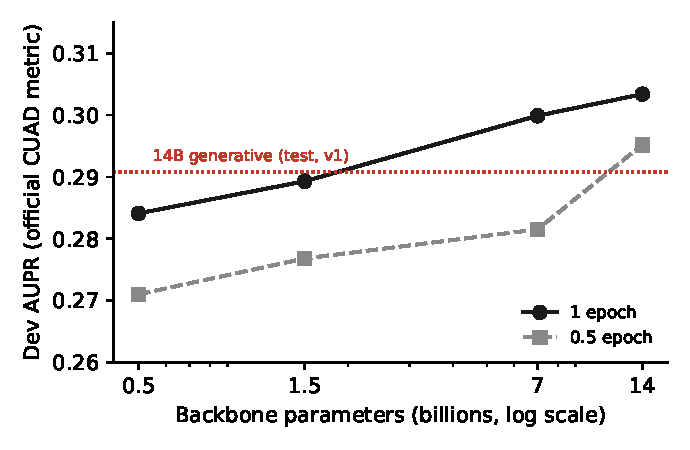
\includegraphics[width=0.72\linewidth]{scaling_curve.pdf}
\caption{Extractive dev AUPR vs.\ backbone size under an identical lean
recipe. A 28x parameter increase yields +0.019 AUPR; the 0.5B extractive
model already matches the 14B generative specialist's test score (dotted
line).}
\label{fig:curve}
\end{figure}

\textbf{Scaling curve.} We trained the identical recipe at four backbone
sizes (Qwen2.5-0.5B/1.5B/7B, Qwen3-14B). Dev AUPR at one epoch: 0.284,
0.289, 0.300, 0.303 (Figure~\ref{fig:curve}). The curve is monotonic and
nearly flat: 28x more parameters buys 1.9 points. The half-billion-parameter
model, trainable overnight on a consumer laptop GPU, already matches the 14B
generative specialist.

\textbf{Test result.} The dev-selected 14B extractive model, scored once on
test, reaches \textbf{0.389} AUPR: +9.8 points over v1 from the framing
change alone. Table~\ref{tab:h2h} shows the head-to-head picture: the
specialist now beats GPT-4o in 25 of 40 categories and GPT-5.2 in 22 of 40,
and beats all four frontier models simultaneously in six categories
(Agreement Date at 0.829 vs.\ best frontier 0.168, Effective Date,
Expiration Date, Document Name, Volume Restriction, Post-Termination
Services).

\begin{table}[t]
\centering
\small
\begin{tabular}{lccccc}
\toprule
Specialist & vs.\ c-4.8 & vs.\ c-4.6 & vs.\ gpt-5.2 & vs.\ gpt-4o & all 4 \\
\midrule
v2 (extractive) & \textbf{8} & \textbf{11} & \textbf{22} & \textbf{25} & \textbf{6} \\
v1 (generative) & 3 & 3 & 11 & 11 & 2 \\
\bottomrule
\end{tabular}
\caption{Categories (of 40 scorable) in which each specialist strictly beats
each frontier model, and the number in which it beats all four
simultaneously.}
\label{tab:h2h}
\end{table}

\textbf{The framing fix reached reasoning categories.} The v1 interpretation
that specialists only learn conventions does not survive v2. Categories that
collapsed under generation recovered sharply under extraction: Covenant Not
To Sue 0.107 to 0.539, Joint IP Ownership 0.184 to 0.500, Anti-Assignment
0.224 to 0.497, Uncapped Liability 0.150 to 0.415. Median category AUPR rose
from 0.219 to 0.340. Generation was taxing the model twice: it had to
reproduce long legal spans verbatim, where a single paraphrased token breaks
Jaccard matching, from a decoder trained for fluency rather than fidelity.
Extraction removes both failure modes by construction.

\section{The Pre-Registered Miss}
\label{sec:miss}

Before any v2 GPU spend we published the prediction that the extractive 14B
clears 0.50 test AUPR, a target informed by the published 0.47 of the
recipe-complete 0.9B DeBERTa-xlarge baseline. The measured 0.389 falls short,
and we report it as a miss. The miss is informative. The scaling curve rules
out backbone capacity as the binding constraint, and the framing comparison
rules out task formulation; what separates our setup from the reference
baseline is the training recipe (single epoch vs.\ multiple, 2:1 negative
subsampling vs.\ full negatives, untuned vs.\ tuned hyperparameters). The
remaining 8 to 17 point gap to the frontier is therefore located in the
cheapest, most controllable part of the pipeline. A recipe-complete v3 is the
planned follow-up, carrying the same 0.50 target forward.

\section{Cost}
\label{sec:cost}

Total project spend was approximately \$577: about \$494 for frontier
baseline evaluations (dominated by Claude at roughly \$165 per full test run
even with prompt caching) and about \$83 for all specialist training,
evaluation, and the size sweep across both versions. The v2 extractive
specialist cost \$32 end to end, including three backbone sizes trained on a
rented A100 and an 0.5B point trained on a consumer laptop GPU. At deployment
time the comparison is starker: a frontier pass over one contract costs on
the order of \$1.60 at Claude pricing, while specialist inference on owned
hardware has effectively zero marginal cost.

\section{Discussion}
\label{sec:discussion}

\textbf{Why the gap is category-shaped.} CUAD scores span agreement against
expert annotation conventions. For convention-bound categories (dates,
document names, notice periods), the correct span boundary is a fact about
the annotators, not about language understanding; it is learnable from
examples and unavailable to zero-shot models regardless of scale. This
explains all three of our scale results at once: the flat specialist curve,
the GPT-4o/GPT-5.2 tie, and the specialist's clean sweeps on convention
categories against models orders of magnitude larger.

\textbf{What frontier scale still buys.} The categories where frontier
models dominate (Parties at 0.954, Source Code Escrow at 0.917) involve
entity aggregation across a document or rare clause types with few training
examples. These resist both the lean recipe and, apparently, the extractive
head at one epoch; whether a recipe-complete specialist closes them is an
open question for v3.

\textbf{For practitioners.} Two operational lessons. First, task framing is
a cheaper lever than model choice: the same backbone asked two different ways
moved 10 points, five times the gap between two frontier generations.
Second, category-level evaluation is not optional: every deployment-relevant
fact in this paper (which model wins where, and by how much) is invisible in
the overall averages of Table~\ref{tab:overall}.

\textbf{Limitations.} Single benchmark and single domain; one training run
per configuration without seed variance; a deliberately lean recipe that
underperforms the published extractive reference; frontier results depend on
one prompt format (mitigated by using the same format for all four models);
frontier snapshots are those served in June--July 2026; and the specialist's
precision at 80\% recall is zero, so these are ranking-quality results, not
high-recall retrieval results, for all models evaluated.

\section{Conclusion}

On CUAD contract clause extraction, an inexpensive fine-tuned specialist
does not beat the best frontier model overall, but the gap is
category-shaped, task framing moves the specialist five times further than a
generation of frontier scaling moved GPT, and 28x specialist scale is worth
two points. We published a pre-registered target and missed it, which
localized the remaining gap to the training recipe, the cheapest variable in
the system. Code, every model's raw predictions, the run journals including
failures, and the trained adapter are public at
\url{https://github.com/ashish24142/nightwing} and
\url{https://huggingface.co/ashish24142/nightwing-14b-cuad-extractive}.

\begin{thebibliography}{9}

\bibitem[Hendrycks et al.(2021)]{hendrycks2021cuad}
Dan Hendrycks, Collin Burns, Anya Chen, and Spencer Ball.
\newblock CUAD: An expert-annotated NLP dataset for legal contract review.
\newblock In \emph{NeurIPS Datasets and Benchmarks}, 2021.

\bibitem[He et al.(2021)]{he2021deberta}
Pengcheng He, Xiaodong Liu, Jianfeng Gao, and Weizhu Chen.
\newblock DeBERTa: Decoding-enhanced BERT with disentangled attention.
\newblock In \emph{ICLR}, 2021.

\bibitem[Hu et al.(2022)]{hu2022lora}
Edward~J. Hu, Yelong Shen, Phillip Wallis, Zeyuan Allen-Zhu, Yuanzhi Li,
Shean Wang, Lu Wang, and Weizhu Chen.
\newblock LoRA: Low-rank adaptation of large language models.
\newblock In \emph{ICLR}, 2022.

\bibitem[Nosek et al.(2018)]{nosek2018preregistration}
Brian~A. Nosek, Charles~R. Ebersole, Alexander~C. DeHaven, and David~T.
Mellor.
\newblock The preregistration revolution.
\newblock \emph{Proceedings of the National Academy of Sciences},
115(11):2600--2606, 2018.

\bibitem[Qwen Team(2024)]{qwen25}
Qwen Team.
\newblock Qwen2.5 technical report.
\newblock \emph{arXiv preprint arXiv:2412.15115}, 2024.

\bibitem[Qwen Team(2025)]{qwen3}
Qwen Team.
\newblock Qwen3 technical report.
\newblock \emph{arXiv preprint arXiv:2505.09388}, 2025.

\bibitem[Rajpurkar et al.(2018)]{rajpurkar2018squad2}
Pranav Rajpurkar, Robin Jia, and Percy Liang.
\newblock Know what you don't know: Unanswerable questions for SQuAD.
\newblock In \emph{ACL}, 2018.

\bibitem[Wolf et al.(2020)]{wolf2020transformers}
Thomas Wolf et al.
\newblock Transformers: State-of-the-art natural language processing.
\newblock In \emph{EMNLP System Demonstrations}, 2020.

\end{thebibliography}

\end{document}
